\documentclass[11pt,a4paper]{article}

\usepackage{geometry}
\usepackage{graphicx, hyperref}
\usepackage[export]{adjustbox}
\usepackage[USenglish]{babel}
\usepackage[utf8]{inputenc}
\usepackage[T1]{fontenc}
\usepackage[usenames,dvipsnames]{color}

\geometry{left=1.5cm, top=0.9cm, right=1.5cm, bottom=1.5cm}

\hypersetup{colorlinks=true,urlcolor=blue}

\begin{document}
    \pagestyle{empty}

    \begin{center}
        \begin{minipage}[b]{3cm}
            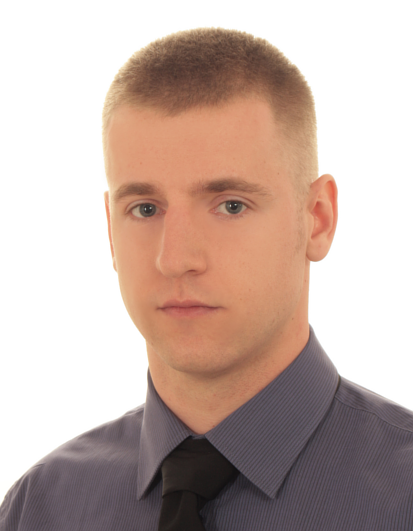
\includegraphics[scale=0.28, right]{photo.png}
        \end{minipage}
        \hspace{0.2cm}
        \begin{minipage}[b]{7cm}
            {\Large \sc Marcin Rainka}
            \begin{description} \itemsep1pt \parskip0pt \parsep0pt
                \item[Address] PCK st. 7/80, 81-621 Gdynia
                \item[Date of birth] 1st December 1989
                \item[Phone number] (+48) 505 464 392
                \item[E-mail] \href{mailto:marcin.rainka@gmail.com}{marcin.rainka@gmail.com}
                \item[LinkedIn] \href{https://linkedin.com/in/marcinrainka}{https://linkedin.com/in/marcinrainka}
            \end{description}
        \end{minipage}
    \end{center}

    \vspace{-0.4cm}

    \noindent\rule{\textwidth}{0.1mm}

    %==================== PROFILE AND OBJECTIVE ====================================================

    \bigskip

    \noindent{\large \bf Profile and objective}

    \smallskip

    \noindent
    Master of~Computer Science with~more than two years of~experience as~a~software developer, familiar with~many technologies, wishing further development and~new challenges.

    %==================== EXPERIENCE ===============================================================

    \bigskip

    \noindent{\large \bf Experience}

    \smallskip

    \noindent{\bf Grupa Wirtualna Polska S.A. -- Junior iOS Developer \hfill September 2016 -- present}
    \vspace{-0.2cm}
    \begin{itemize} \itemsep1pt \parskip0pt \parsep0pt
        \item Developing iOS applications
        \item Writing automated tests
    \end{itemize}
    \vspace{-0.2cm}
    \noindent{\bf AIC S.A. -- Software Developer \hfill April 2014 -- August 2016}
    \vspace{-0.2cm}
    \begin{itemize} \itemsep1pt \parskip0pt \parsep0pt
        \item Developing mobile for~iOS, desktop for~Windows (WPF) and~web applications (AngularJS)
        \item Development of project called iProd, controlling automatic production line with iPads
        \item Creating REST APIs in Python
        \item Writing automated tests and documentation
    \end{itemize}

    %==================== EDUCATION ================================================================

    \medskip
  
    \noindent{\large \bf Education}
  
    \smallskip

    \noindent{{\bf University of Gdańsk}, Faculty of Mathematics, Physics and Informatics \hfill {\bf 2012 -- 2014}}
    \vspace{-0.2cm}
    \begin{itemize} \itemsep1pt \parskip0pt \parsep0pt
        \item[ ] M.Sc in Computer Science degree (daily studies)
    \end{itemize}
    \vspace{-0.2cm}
    \noindent{{\bf University of Warmia and Mazury}, Faculty of Mathematics and Computer Science \hfill {\bf 2008 -- 2012}}
    \vspace{-0.2cm}
    \begin{itemize} \itemsep1pt \parskip0pt \parsep0pt
        \item[ ] B.Eng in Computer Science degree (daily studies)
    \end{itemize}
    \vspace{-0.2cm}
    \noindent{\bf High School No I in Mrągowo \hfill 2005 -- 2008}
    \vspace{-0.2cm}
    \begin{itemize} \itemsep1pt \parskip0pt \parsep0pt
        \item[ ] Mathematics-Physics-Informatics
    \end{itemize}

    %==================== COURSES ==================================================================

    \medskip

    \noindent{\large \bf Additional qualifications}

    \smallskip

    \noindent{Autotesting | Bottega IT Solutions \hfill {\bf April 2015}}

    \noindent{Craftsmanship, patterns and architecture for iOS developers | Bottega IT Solutions \hfill {\bf October 2014}}
  
    %==================== TECHNICAL SKILLS =========================================================
  
    \vspace{0.3cm}
    \noindent{\Large \bf Technical skills}
  
    %---------- Programming/markup languages -------------------------------------------------------
  
    \medskip
    \noindent{\large \bf Programming/markup languages}
  
    \medskip
    \centerline{
        \hfill
        $\bullet$ C++
        {
            \color{Gray}
            \framebox[36pt]{
                \color{Black}
                \rule{3pt}{7pt} \rule{3pt}{7pt} \rule{3pt}{7pt} \rule{3pt}{7pt}
                \color{Gray}
                \rule{3pt}{7pt}
            }
        }
        \hfill
        $\bullet$ Java
        {
            \color{Gray}
            \framebox[36pt]{
                \color{Black}
                \rule{3pt}{7pt} \rule{3pt}{7pt} \rule{3pt}{7pt}
                \color{Gray}
                \rule{3pt}{7pt} \rule{3pt}{7pt}
            }
        }
        \hfill
        $\bullet$ HTML \& CSS
        {
            \color{Gray}
            \framebox[36pt]{
                \color{Black}
                \rule{3pt}{7pt} \rule{3pt}{7pt} \rule{3pt}{7pt} \rule{3pt}{7pt}
                \color{Gray}
                \rule{3pt}{7pt}
            }
        }
        \hfill
        $\bullet$ TeX
        {
            \color{Gray}
            \framebox[36pt]{
                \color{Black}
                \rule{3pt}{7pt} \rule{3pt}{7pt} \rule{3pt}{7pt}
                \color{Gray}
                \rule{3pt}{7pt} \rule{3pt}{7pt}
            }
        }
        \hfill
    }
  
    %---------- Code editors -----------------------------------------------------------------------
  
    \bigskip
    \noindent{\large \bf Code editors}
  
    \medskip
    \centerline{
        \hfill
        $\bullet$ Vim
        \hfill
        $\bullet$ Eclipse
        \hfill
        $\bullet$ Visual Studio
        \hfill
        $\bullet$ Dev-C++
        \hfill
        $\bullet$ Geany
        \hfill
        $\bullet$ Notepad++
        \hfill
    }
  
    \bigskip
    \noindent
    \begin{minipage}[t]{0.35\textwidth}
  
        %---------- Operating systems --------------------------------------------------------------
        
        \noindent{\large \bf Operating systems}
        
        \medskip
        \centerline{
            \hfill
            $\bullet$ Linux
            \hfill
            $\bullet$ Windows
            \hfill
        }
    \end{minipage}
    \begin{minipage}[t]{0.65\textwidth}
  
        %---------- Graphics software and office suite ---------------------------------------------
        
        \noindent{\large \bf Graphics software and office suite}
        
        \medskip
        \centerline{
            \hfill
            $\bullet$ Gimp
            \hfill
            $\bullet$ Blender
            \hfill
            $\bullet$ LibreOffice
            \hfill
            $\bullet$ OpenOffice
            \hfill
        }
    \end{minipage}
  
    %---------- Others -----------------------------------------------------------------------------
  
    \bigskip
    \noindent{\large \bf Others:}
    \vspace{-1mm}
    \begin{itemize} \itemsep2pt \parskip0pt \parsep0pt
        \item[--] object-oriented programming;
        \item[--] basic knowledge of SDL (Simple DirectMedia Layer) library;
        \item[--] basics of CUDA and parallel computing;
        \item[--] creating Git repositories;
        \item[--] touch-typing.
    \end{itemize}
  
    %==================== INTERESTS AND HOBBIES ====================================================
  
    \vspace{0.3cm}
    \noindent{\Large \bf Interests and hobbies}
  
    \medskip
    \centerline{
        \hfill
        $\bullet$ Powerlifting
        \hfill
        $\bullet$ Drawing
        \hfill
        $\bullet$ Computer graphics
        \hfill
        $\bullet$ Game development
        \hfill
    }
  
    %==================== MISCELLANEOUS ============================================================
  
    \vspace{0.5cm}
    \noindent{\Large \bf Miscellaneous}
  
    \medskip
    \centerline{
        \hfill
        $\bullet$ English B2 (Upper-Intermediate)
        \hfill
        $\bullet$ Driving licence B
        \hfill
    }
  
    %==================== CLAUSE ===================================================================
  
    \vspace{0.92cm}
    \noindent \textit{''I hereby give consent for my personal data to be processed for the~purposes
    of recruitment,\linebreak in accordance with the~Personal Data Protection Act dated 29.08.1997
    (uniform text: Journal of Laws of the~Republic of Poland 2002 No 101, item 926
    with further amendments).''}
\end{document}
